\chapter{HTTP protocol}
HTTP protocol was presented for the first time in the RFC 1945 (Request for Comment).\\
The Hypertext Transfer Protocol (HTTP) is an application-level protocol with the lightness and speed necessary for distributed, collaborative, hypermedia information systems. It is a generic, stateless, object-oriented protocol which can be used for many tasks, such as name servers and distributed object management systems, through extension of its request methods (commands).\\
It's not the first Hypertext protocol in history because there was Hypertalk, made by Apple before. \\
A feature of HTTP is the typing of data representation, allowing systems to be built independently f the data being transferred. HTTP has been in use by the World-Wide Web global information initiative since 1990.

\section{Terminology}
\begin{itemize}
\item{\textbf{connection}\\
a transport layer virtual circuit established between two application programs for the purpose of communication.}
\item{\textbf{message}\\
the basic unit of HTTP communication, consisting of a structured sequence of octets matching the syntax defined in Section 4 and transmitted via the connection.}
\item{\textbf{request}\\
an HTTP request message.
}
\item{\textbf{response}\\
an HTTP response message.}
\item{\textbf{resource}\\
a network data object or service which can be identified by a URI.}
\item{\textbf{entity}\\
a particular representation or rendition of a data resource, or reply from a service resource, that may be enclosed within a request or response message. An entity consists of metainformation in the form of entity headers and content in the form of an entity body.}
\item{\textbf{client}\\
an application program that establishes connections for the purpose of sending requests.}
\item{\textbf{user agent}\\
the client which initiates a request. These are often browsers, editors, spiders (web-traversing robots), or other end user tools.}
\item{\textbf{server}\\
an application program that accepts connections in order to service requests by sending back responses.}
\item{\textbf{origin server}\\
the server on which a given resource resides or is to be created.}
\item{\textbf{proxy}\\
an intermediary program which acts as both a server and a client for the purpose of making requests on behalf of other clients. Requests are serviced internally or by passing them, with possible translation, on to other servers. A proxy must interpret and, if necessary, rewrite a request message before forwarding it.\\
Proxies are often used as client-side portals
through network firewalls and as helper applications for handling requests via protocols not implemented by the user agent.}
\item{\textbf{gateway}\\
a server which acts as an intermediary for some other server. Unlike a proxy, a gateway receives requests as if it were the origin server for the requested resource; the requesting client may not be aware that it is communicating with a gateway.\\
Gateways are often used as server-side portals through network firewalls and as protocol translators for access to resources stored on non-HTTP systems.}
\item{\textbf{tunnel}\\
a tunnel is an intermediary program which is acting as a blind relay between two connections. Once active, a tunnel is not considered a party to the HTTP communication, though the tunnel may have been initiated by an HTTP request. The tunnel ceases to exist when both ends of the relayed connections are closed.\\
Tunnels are used when a portal is necessary and the intermediary cannot, or should not, interpret the relayed communication.}
\item{\textbf{cache}\\
a program's local store of response messages and the subsystem that controls its message storage, retrieval, and deletion. A cache stores cachable responses in order to reduce the response time and network bandwidth consumption on future, equivalent requests. Any client or server may include a cache, though a cache cannot be used by a server while it is acting as a tunnel.}
\end{itemize}
Any given program may be capable of being both a client and a server; our use of these terms refers only to the role being performed by the program for a particular connection, rather than to the program's capabilities in general. Likewise, any server may act as an origin server, proxy, gateway, or tunnel, switching behavior based on the nature of each request.

\section{Basic rules}
The following rules are used throughout are used to describe the grammar used in the RFC 1945.
\begin{table}[h]
\centering
\footnotesize
\begin{tabular}{rl}
\textbf{OCTET =}& <any 8-bit sequence of data>\\
\textbf{CHAR =}& <any US-ASCII character (octets 0 - 127)>\\
\textbf{UPALPHA =}& <any US-ASCII uppercase letter "A".."Z">\\
\textbf{LOALPHA =}& <any US-ASCII lowercase letter "a".."z">\\
\textbf{ALPHA =}& UPALPHA | LOALPHA\\
\textbf{DIGIT =}& <any US-ASCII digit "0".."9">\\
\textbf{CTL =}& <any US-ASCII control character (octets 0 - 31) and DEL (127)>\\
\textbf{CR =}& <US-ASCII CR, carriage return (13)>\\
\textbf{LF =}& <US-ASCII LF, linefeed (10)>\\
\textbf{SP =}& <US-ASCII SP, space (32)>\\
\textbf{HT =}& <US-ASCII HT, horizontal-tab (9)>\\
\textbf{<"> =}& <US-ASCII double-quote mark (34)>\\
\end{tabular}
\end{table}

\section{Messages}
\subsection{Different versions of HTTP protocol}
\begin{itemize}
\item{\textbf{HTTP/0.9 Messages}\\
Simple-Request and Simple-Response do not allow the use of any header information and are limited to a single request method (GET).\\ Use of the Simple-Request format is discouraged because it prevents the server from identifying the media type of the returned entity.
\begin{center}
\begin{tabular}{c}
\begin{lstlisting}[linewidth=240pt, basicstyle=\footnotesize\sffamily,]
HTTP-message = Simple-Request | Simple-Response
\end{lstlisting}
\end{tabular}
\end{center}
\begin{center}
\begin{tabular}{c}
\begin{lstlisting}[linewidth=230pt, basicstyle=\footnotesize\sffamily,]
Simple-Request  = "GET" SP Request-URI CRLF


Simple-Response = [ Entity-Body ]
\end{lstlisting}
\end{tabular}
\end{center}
}
\item{\textbf{HTTP/1.0 Messages}\\
Full-Request and Full-Response use the generic message format of RFC 822 for transferring entities. Both messages may include optional header fields (also known as "headers") and an entity body. The entity body is separated from the headers by a null line (i.e., a line with nothing preceding the CRLF).
\begin{center}
\begin{tabular}{c}
\begin{lstlisting}[linewidth=230pt, basicstyle=\footnotesize\sffamily,]
HTTP-message = Full-Request | Full-Response
\end{lstlisting}
\end{tabular}
\end{center}
\begin{center}
\begin{tabular}{c}
\begin{lstlisting}[linewidth=340pt, basicstyle=\footnotesize\sffamily,]
Full-Request = Request-Line
               *(General-Header | Request-Header | Entity-Header)
               CRLF
               [Entity-Body]
               
               
Full-Response = Status-Line
                *(General-Header | Request-Header | Entity-Header)
                CRLF
                [Entity-Body]               
\end{lstlisting}
\end{tabular}
\end{center}
}
\end{itemize}

\subsection{Headers}
The order in which header fields are received is not significant. However, it is "good practice" to send General-Header fields first, followed by Request-Header or Response-Header fields prior to the Entity-Header fields.\\
Multiple HTTP-header fields with the same field-name may be present in a message if and only if the entire field-value for that header field is defined as a comma-separated list.
\begin{center}
\begin{tabular}{c}
\begin{lstlisting}[linewidth=260pt, basicstyle=\footnotesize\sffamily,]
HTTP-header = field-name ":" [ field-value ] CRLF
\end{lstlisting}
\end{tabular}
\end{center}

\subsection{Request-Line}
\begin{center}
\begin{tabular}{c}
\begin{lstlisting}[linewidth=320pt, basicstyle=\footnotesize\sffamily,]
Request-Line = Method SP Request-URI SP HTTP-Version CRLF

Method         = "GET" | "HEAD" | "POST" | extension-method

extension-method = token
\end{lstlisting}
\end{tabular}
\end{center}
The list of methods acceptable by a specific resource can change dynamically; the client is notified through the return code of the response if a method is not allowed on a resource.\\
Servers should return the status code 501 (not implemented) if the method is unrecognized or not implemented.

\subsection{Request-URI}
The Request-URI is a Uniform Resource Identifier and identifies the resource upon which to apply the request.
\begin{center}
\begin{tabular}{c}
\begin{lstlisting}[linewidth=190pt, basicstyle=\footnotesize\sffamily,]
Request-URI = absoluteURI | abs_path
\end{lstlisting}
\end{tabular}
\end{center}
The absoluteURI form is only allowed when the request is being made to a proxy. The proxy is requested to forward the request and return the response. If the request is GET or HEAD and a prior response is cached, the proxy may use the cached message if it passes any restrictions in the Expires header field.\\
Note that the proxy may forward the request on to another proxy or directly to the server specified by the absoluteURI. In order to avoid request loops, a proxy must be able to recognize all of its server names, including any aliases, local variations, and the numeric IP address.\\\\
The most common form of Request-URI is that used to identify a resource on an origin server or gateway. In this case, only the absolute path of the URI is transmitted.

\subsection{Request Header}
The request header fields allow the client to pass additional information about the request, and about the client itself, to the server.\\
These fields act as request modifiers, with semantics equivalent to the parameters on a programming language method (procedure) invocation.
\begin{center}
\begin{tabular}{c}
\begin{lstlisting}[linewidth=410pt, basicstyle=\footnotesize\sffamily,]
Request-Header = Authorization | From | If-Modified-Since | Referer | User-Agent
\end{lstlisting}
\end{tabular}
\end{center} 

\subsection{Status line}
\begin{center}
\begin{tabular}{c}
\begin{lstlisting}[linewidth=330pt, basicstyle=\footnotesize\sffamily,]
Status-Line = HTTP-Version SP Status-Code SP Reason-Phrase CRLF
\end{lstlisting}
\end{tabular}
\end{center}
\begin{table}[h]
\centering
\footnotesize
\begin{tabular}{|r|l|}
\multicolumn{2}{c}{\textbf{General Status code}}\\
\hline
\textbf{1xx: Informational} & {Not used, but reserved for future use}\\
\hline
\textbf{2xx: Success}&{The action was successfully received,}\\
\hline
& {understood, and accepted.}\\
\hline
\textbf{3xx: Redirection} & {Further action must be taken in order to}\\
&{complete the request}\\
\hline
\textbf{4xx: Client Error}&{The request contains bad syntax or cannot}\\
&{be fulfilled}\\
\hline
\textbf{5xx: Server Error}&{The server failed to fulfill an apparently}\\
&{valid request}\\
\hline
\end{tabular}
\end{table}
\begin{table}[h]
\centering
\footnotesize
\begin{tabular}{|r|l|}
\multicolumn{2}{c}{\textbf{Known service code}}\\
\hline
\textbf{200}&{OK}\\
\hline
\textbf{201}&{Created}\\
\hline
\textbf{202}&{Accepted}\\
\hline
\textbf{204}&{No Content}\\
\hline
\textbf{301}&{Moved Permanently}\\
\hline
\textbf{302}&{Moved Temporarily}\\
\hline
\textbf{304}&{Not Modified}\\
\hline
\textbf{400}&{Bad Request}\\
\hline
\textbf{401}&{Unauthorized}\\
\hline
\textbf{403}&{Forbidden}\\
\hline
\textbf{404}&{Not Found}\\
\hline
\textbf{500}&{Internal Server Error}\\
\hline
\textbf{501}&{Not Implemented}\\
\hline
\textbf{502}&{Bad Gateway}\\
\hline
\textbf{503}&{Service Unavailable}\\
\hline
\end{tabular}
\end{table}

\vspace{10cm}
\section{Examples}
The following pieces of code are examples of TCP client connection to \textbf{www.google.it}, using functions explained in Chapter \ref{networkC}.
\subsection{HTTP 0.9}
The following piece of code define a structure, used to connect to Google server. 

The most important thing is that \textbf{socket()} is entry-point for level 4, but also \textbf{connect()} is the request to Kernel to extablish the connection.\\ \textbf{read()} and \textbf{write()} are system calls used respectively to obtain result(response) of a request and to generate request.\\ These function permit us to ask to lower level to do this things, without knowing content of system buffers (stream). The second part is only used to read the input.

\subsection{HTTP 1.0}
The protocol has no mandatory headers to be added in the request field. This protocol is compliant with HTTP 0.9.
To keep the connection alive, "Connection" header with "keep-alive" as header field must be added to request message. The server, receiving the request, replies with a message with the same header value for "Connection".\\
This is used to prevent the closure of the connection, so if the client needs to send another request, he can use the same connection.
This is usually used to send many files and not only one.\\
The connection is kept alive until either the client or the server decides that the connection is over and one of them drops the connection. If the client doesn't send new requests to the server, the second one usually drops the connection after a couple of minutes.\\
The client could read the response of request, with activated keep alive option, reading only header and looking to "Content-length" header field value to understand the length of the message body. This header is added only if a request with keep-alive option is done.\\
This must be done because we can't look only to empty system stream, because it could be that was send only the response of the first request or a part of the response.\\
Otherwise, when the option keep alive is not used, the client must fix a max number of characters to read from the specific response to his request, because it doesn't know how many character compose the message body.

\subsection{HTTP 1.1}
It has by default the option keep alive actived by default with respect to HTTP 1.0. It has the mandatory header "Host" followed by the hostname of the remote system to which the request or the response is sent. The body is organized in chunks, so we need the connection kept alive to manage future new chunks.\\
This is useful with dynamic pages, in which the server doesn't know the length of the stream in advance and can update the content of the stream during the extablished connection, sending a fixed amount of bytes to client. We can check if the connection is chunked oriented, looking for the header "Transfer-Encoding" with value "chunked".\\ 
Each connection is composed by many chunks and each of them is composed by chunk length followed by chunk body, except for the last one that has length 0 (see Figure \ref{chunked_body}). The following grammar represents how the body is organized:
\begin{center}
\begin{tabular}{c}
\begin{lstlisting}[linewidth=320pt, basicstyle=\footnotesize\sffamily,]
Chunked-Body   = *chunk
                 last-chunk
                 trailer
                 CRLF

chunk          = chunk-size [ chunk-extension ] CRLF
                 chunk-data CRLF

chunk-size     = 1*HEX
last-chunk     = 1*("0") [ chunk-extension ] CRLF

chunk-extension= *( ";" chunk-ext-name [ "=" chunk-ext-val ] )

chunk-ext-name = token
chunk-ext-val  = token | quoted-string
chunk-data     = chunk-size(OCTET)
trailer        = *(entity-header CRLF)
\end{lstlisting}
\end{tabular}
\end{center}

\begin{figure}[h]
\centering
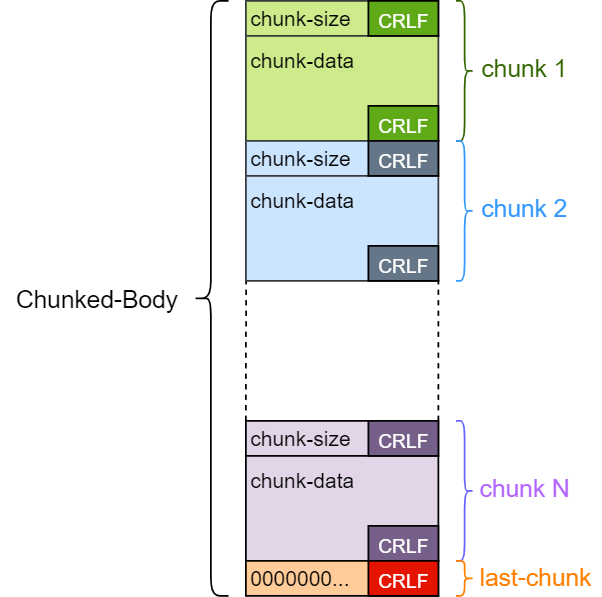
\includegraphics[scale=0.5]{Images/HTTP/Chunked-Body}\caption{\footnotesize{Chunked body.}}\label{chunked_body}
\end{figure}